\documentclass{article}
\usepackage[paperwidth=170mm,paperheight=141mm,margin=2mm]{geometry}
\usepackage{fontspec}
\usepackage{type1cm}
\usepackage{xcolor}
\definecolor{sourcebar}{RGB}{95,95,95}
\usepackage{graphicx}
\usepackage{tcolorbox}
\tcbuselibrary{skins}
\setmainfont{TeX Gyre Termes}
\pagestyle{empty}
\setlength{\parindent}{0pt}
\setlength{\parskip}{0pt}
\newlength{\framegroupwidth}
\newcommand{\bodyfont}{\fontsize{11.4pt}{13pt}\selectfont}
\tcbset{
  roundedgrayframe/.style={
    enhanced,
    arc=2mm,
    boxrule=0.6pt,
    colframe=gray!30!black,
    colback=gray!4,
    left=6mm,
    right=6mm,
    top=2.4mm,
    bottom=2mm,
    boxsep=0pt,
    fonttitle=\bfseries\fontsize{12pt}{13pt}\selectfont,
    coltitle=white,
    colbacktitle=sourcebar,
    toptitle=1.6mm,
    bottomtitle=1.6mm,
    titlerule=0pt
  }
}
\begin{document}
\graphicspath{{assets/}}
\vspace*{-0.6mm}
\begin{tcolorbox}[roundedgrayframe,title={Box 4. Example of Human Behavior VQA: Using Scooter}]
{\bodyfont
\textbf{Frames:}\par
\vspace{0.8mm}
\begin{center}
\setlength{\framegroupwidth}{0.90\linewidth}
\begin{minipage}{\framegroupwidth}
\centering
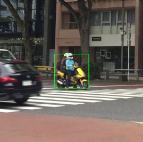
\includegraphics[width=0.195\linewidth]{assets/frame-01.png}\hspace{0.006\linewidth}%
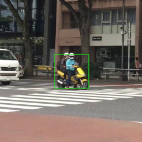
\includegraphics[width=0.195\linewidth]{assets/frame-02.png}\hspace{0.006\linewidth}%
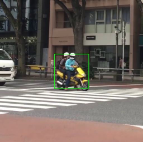
\includegraphics[width=0.195\linewidth]{assets/frame-03.png}\hspace{0.006\linewidth}%
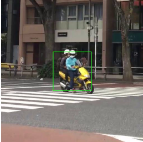
\includegraphics[width=0.195\linewidth]{assets/frame-04.png}\hspace{0.006\linewidth}%
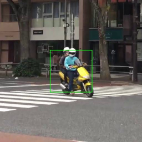
\includegraphics[width=0.195\linewidth]{assets/frame-05.png}
\end{minipage}
\end{center}
\vspace{1.2mm}
\textbf{System Prompt:} You are an expert pedestrian behavior labeler, specializing in analyzing pedestrians’ behavior on the road. You will perform visual analysis on multiple sequential images over time.\par
\vspace{1.4mm}
\textbf{Question 1:} The images show a pedestrian in a bounding box with surrounding context. The image is a cropped frame from a car’s front camera.\par
Is the pedestrian \textcolor{red}{using a scooter}?\par
Please answer y or n, only one letter.\par
\vspace{3mm}
\textbf{Answer:} y\par
\vspace{4.2mm}
\noindent\textcolor{black!55}{\rule{\linewidth}{0.6pt}}\par
\vspace{2.5mm}
\textbf{Question 2:} The images show a pedestrian in a bounding box with surrounding context. The image is a cropped frame from a car’s front camera.\par
The pedestrian is \textcolor{red}{not using a scooter}. Is this statement correct?\par
Please answer y or n, only one letter.\par
\vspace{3mm}
\textbf{Answer:} n
}
\end{tcolorbox}
\end{document}
